\subsection{ADI algorithm}
\subsubsection{Generation of representative set of IMG\_LM data: planetary system}
Using a combination of the HEEPS code and the ScopeSim code with the METIS package we have performed simulations of a star and a point source companion in order to test critical algorithms for high contrast imaging on simulated data of METIS.
Using the HEEPS code we simulate a sequence of up to 12000 PSFs of an unresolved star behind the RAVC coronagraph and of an unresolved companion sufficiently far away from the coronagraph to be considered off-axis, with each PSF corresponding with an integration time of 300 milliseconds for a total of 3600 seconds of observing time. Each PSF is generated with a (SCAO-only) wavefront sampled every 300 ms (comparable to the coherence time t0 at L-band), thereby effectively time sampling the atmospheric wavefront aberrations. Both PSFs are scaled to the magnitude of the parent star ($L=3.5$). For this demonstration we use a time sequence of 12000 PSFs but will apply some windowing and temporal binning to increase execution speed on a laptop. 
The two PSFs are combined together with an offset of 100 mas, an additional delta magnitude ($\Delta L=7.7$) for the companion and field rotation over 1 hour (corresponding with 30 degrees change in position angle). The system could be described at Beta Pic b orbiting at 100 mas around its host star. A second source is added at opposite position angle to see the symmetry of the reduction (of use for the APP coronagraph which only has one dark hole). This combined source is fed into ScopeSim as a fits file with the WCS information conveying the spatial extent. The coronagraphic transmissions are transferred to ScopeSim as well during this process.
In the ScopeSim step the instrumental noise and background expected from both METIS and ELT is injected and the source flux reduced according to system transmission. 
After these processing steps we are left with a large 3D cube of a star (x, y, time) with two planets undergoing field rotation which we use for the ADI processing step using the VIP\_HCI package. For this example, the output images have been truncated to 201x201 pixels and the images have been binned to 30 seconds exposure time ($N_\mathrm{bin}=100$) to further reduce execution time.
\subsubsection{Demonstration of ADI algorithm on simulated IMG\_LM data}
The most basic PSF subtraction of VIP\_HCI is the standard ADI algorithm from Marois et al 2006, where the median of the cube is first subtracted and in a second step optimally-scaled time-localized medians are subtracted in annular rings. Afterwards each image in the cube is derotated with the known position angle. Subsequently the derotated and PSF subtracted images are averaged to give a final stacked version. When the second annular optimized subtraction step is skipped this procedure is equal to the one described in the PIP Spec.
For the LMS IFU, this ADI procedure can similarly be followed for each wavelength in the reduced cubes. In VIP\_HCI it is possible to do a two-step (first ADI then SDI) or single-step reduction, in which rescaled images from other wavelength slices are used to provide additional PSF reference material.
Example output images for ADI reduction for LM RAVC data.


\begin{figure}[!ht]
  \centering
  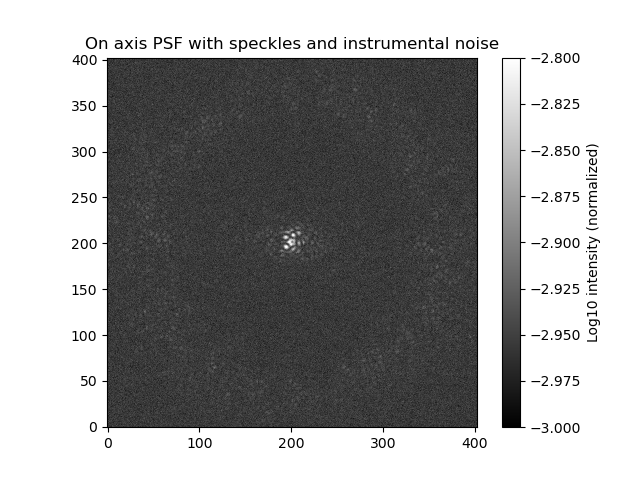
\includegraphics[width=0.6\textwidth]{./figures/onaxis_psf.png}
  \caption{On-axis coronagraphic PSF with instrumental noise injected and with corrected atmospheric turbulence. The circular control region from the AO system is clearly visible.}
  %\label{fig:metis_l}
\end{figure}
\begin{figure}[!ht]
  \centering
  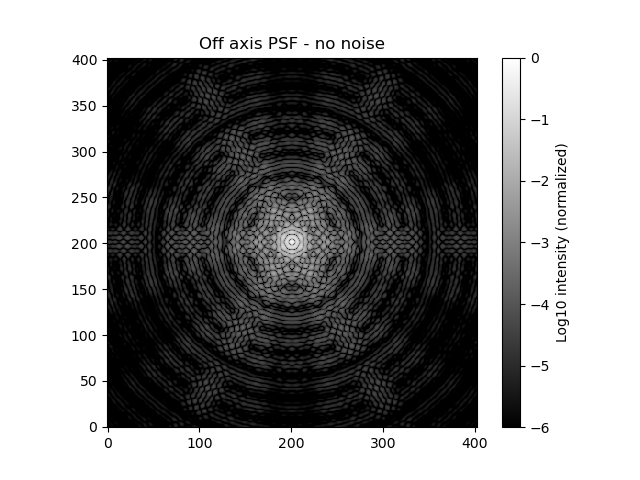
\includegraphics[width=0.6\textwidth]{./figures/offaxis_psf.png}
  \caption{Off-axis PSF without instrumental noise.}
  %\label{fig:metis_l}
\end{figure}

\begin{figure}[!ht]
  \centering
  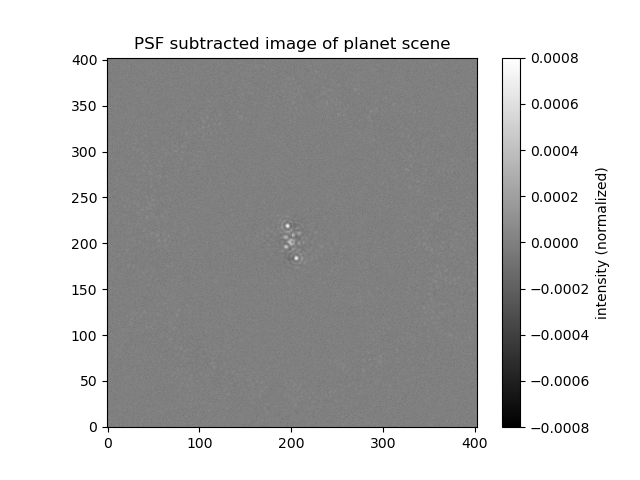
\includegraphics[width=0.6\textwidth]{./figures/adi_meansub.png}
  \caption{Single frame of image stack with mean PSF subtracted.}
  %\label{fig:metis_l}
\end{figure}

\begin{figure}[!ht]
  \centering
  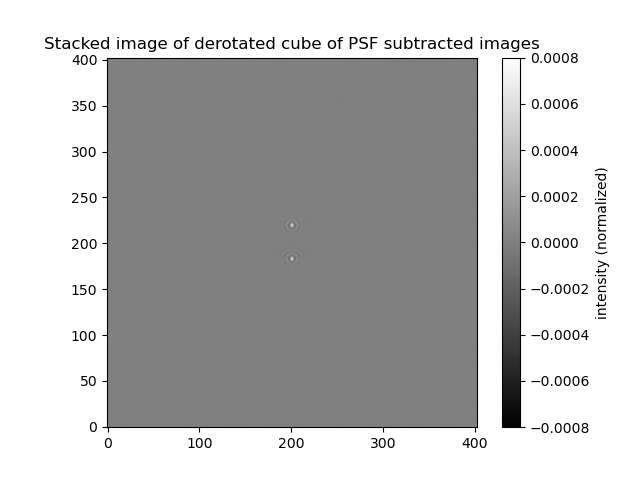
\includegraphics[width=0.6\textwidth]{./figures/adi_derotstack.png}
  \caption{Derotated stack of ADI reduced images.}
  %\label{fig:metis_l}
\end{figure}

Additionally, the contrast curves can be extracted (raw contrast over time-averaged cube, 5 sigma contrast after ADI processing). Please note that the plotted contrast is dependent on the assumptions made for this demonstration (SCAO-only effects, no additional jitter / pupil drifts / no residual atmospheric dispersion, 120 binned frames with each 100 frames of 0.3s integration time, 30 degrees image rotation). 
Injection and retrieval of point sources of known intensity is performed to calculate the efficiency or throughput of the ADI post-processing technique. Closer to the star the same amount of position angle movement will be seen as an increasingly smaller physical movement. Therefore, self-subtraction of a point source signal will be more pronounced and increased losses are seen close to the star. The following plot shows the post-processing only component of the ADI reduction losses. The radial coronagraphic throughput losses due to partial suppression of off-axis sources will be provided separately (and is not included in these sensitivity plots for this example).



Following the SNR definitions of Mawet et al 2014 the noise is calculated in annular rings and corrected for the relatively low number of effective samples. A 5-sigma sensitivity curve is produced by injection and retrieval of sources. In addition, a post-ADI SNR map is generated. Note that the two injection planets are so bright that an unmasked SNR map gives an underestimated SNR as their presence strongly alters the local noise estimate. Nonetheless they are both recognized as significant detections.

\begin{figure}[!ht]
  \centering
  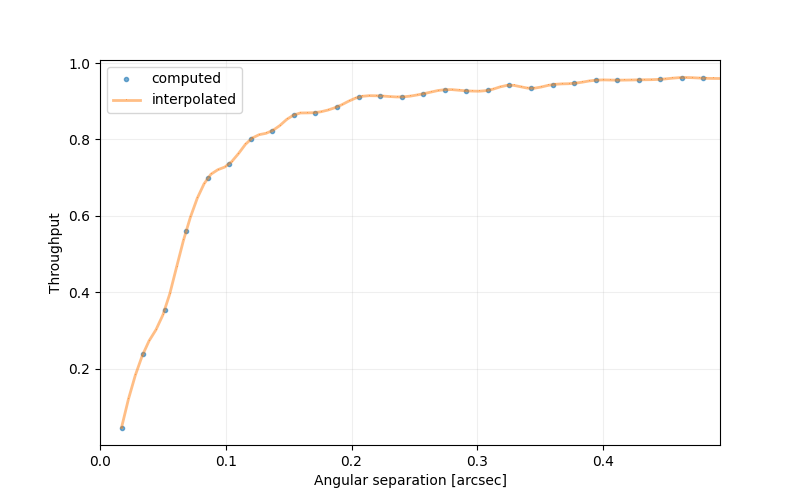
\includegraphics[width=0.6\textwidth]{./figures/adi_throughput.png}
  \caption{Efficiency of ADI algorithm in retrieving inserted point sources as a function of angular separation.}
  %\label{fig:metis_l}
\end{figure}

\begin{figure}[!ht]
  \centering
  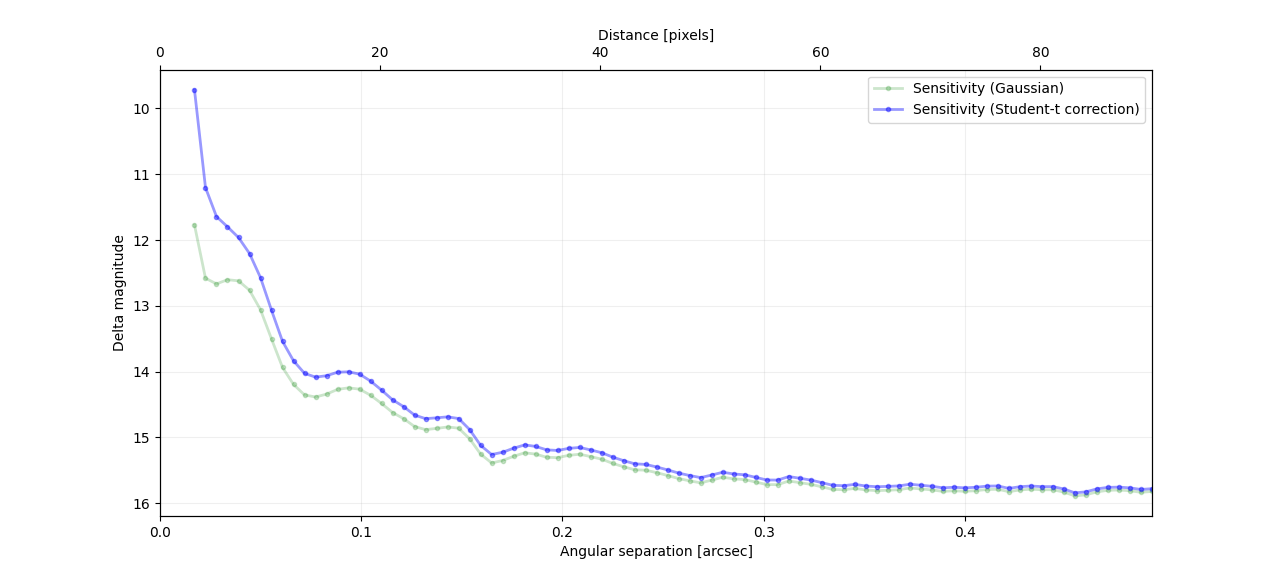
\includegraphics[width=0.6\textwidth]{./figures/adi_contrast.png}
  \caption{Achievable contrast for the $L=3.5$ target in 1 hour integration time as a function of angular separation.}
  %\label{fig:metis_l}
\end{figure}

\begin{figure}[!ht]
  \centering
  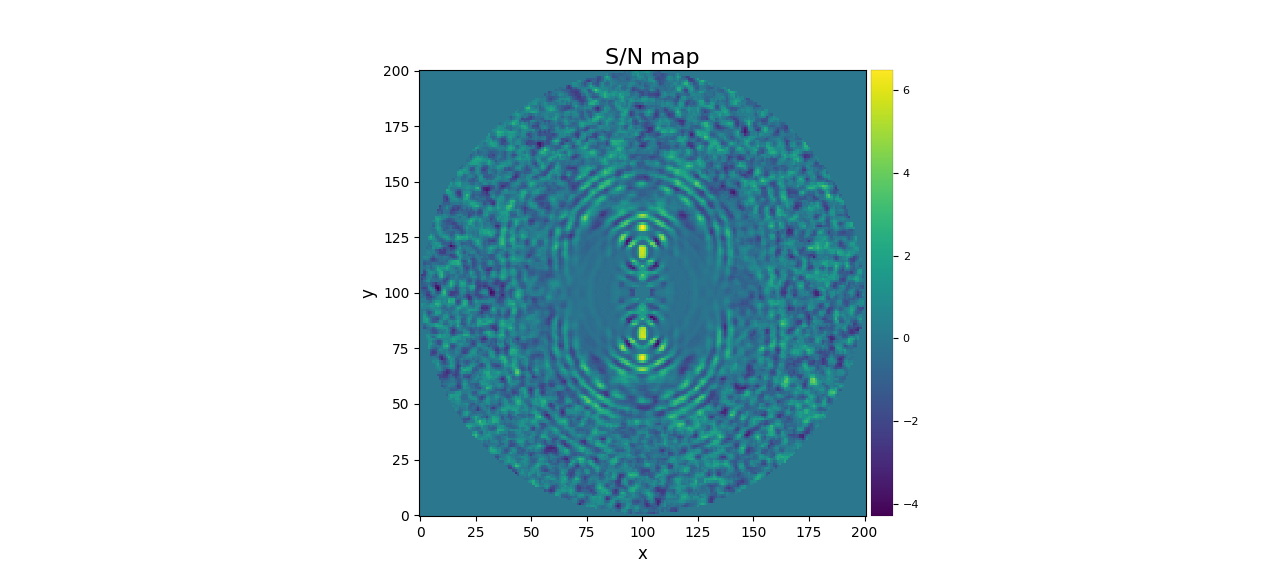
\includegraphics[width=0.6\textwidth]{./figures/adi_snrmap.png}
  \caption{Two dimensional ADI map of post ADI signal to noise of point sources. Two point sources that were inserted at 100 mas are seen.}
  %\label{fig:metis_l}
\end{figure}

\subsubsection{Generation of representative set of IFU data}

To demonstrate the ADI/SDI reduction of an IFU dataset which contains spatial, temporal and spectral information we first generate a METIS IFU HCI dataset of 12000 frames by X by Y pixels and Z spectral bins. Each frame corresponds with an exposure time of 0.3 seconds, with a total integration time of 1 hour. At a central wavelength of 3.8 micron this means approximately X by X lambda/D. 
We generate PSFs with the HEEPS python code in L band with the RAVC coronagraph at a pixel scale of X by X mas. This data is FFT interpolated with VIP\_HCI with a scaling factor to generate 1600 spectral bins in a wavelength range of X micron at a wavelength of X micron.
As the METIS IFU projected on-sky has rectangular pixels we reinterpolate this data for each temporal and spectral slice to a grid of X by X mas and then average the data in one dimension to get a pixel scale of 8.2 by 21 mas. The sum of all flux is set to be equal to the total photons of the star in L-band.
To go back to square pixels, we duplicate the undersampled axis. We inject noise according to the shot noise of the source, sky background and detector read noise with a single resolution element spanning about x by x pixels, while also using a binning factor of X spectrally and Y temporally to reduce memory consumption.



 


\subsubsection{Demonstration of ADI+SDI algorithm on IFU data}


This dataset if used together with an array containing a set of position angles given 1 hour of sky rotation and an array containing the wavelengths of the spectral axis to perform a median PSF subtraction technique using VIP\_HCI on the generated data. This is a two-step process where first for each timestep all spectral slices are rescaled to be on the same lambda/D grid. Then the median of the cube in the spectral dimension is subtracted. This is repeated for every timestep to give a time varying array of residuals. For this array the median in time is also calculated and subtracted. Afterwards the residuals are derotated and stacked. 